%!TEX root = ../dissertation.tex
%\begin{savequote}[75mm]
%Nulla facilisi. In vel sem. Morbi id urna in diam dignissim feugiat. Proin molestie tortor eu velit. Aliquam erat volutpat. Nullam ultrices, diam tempus vulputate egestas, eros pede varius leo.
%\qauthor{Quoteauthor Lastname}
%\end{savequote}
%\label{Data}
\chapter{Methodology}
% Add a paragraph introducing this section

This chapter will provide an overview of the data collection, augmentation, and pre-processing steps (Section \ref{sec:3-data}), followed by the primary implementation frameworks used (Section \ref{sec:3-frameworks}). It will cover details of the \acrshort{NMT} architecture and training methodology (Section \ref{sec:3-model}), before explaining the transfer learning implementation (Section \ref{sec:3-transfer_learning}) and translation evaluation metrics (Section \ref{sec:3-evaluating}).


%, followed by the architectures considered for the model design in \ref{sec:3-architectures}

\newpage

\section{Data}
\label{sec:3-data}
\subsection{Available Datasets}

%Add some text here to talk about the data

The datasets that have been retrieved for use in the translation models have been split into three broad categories to reflect the type of vocabulary and sentence structure that can be expected from each dataset. They are described as follows:

\begin{itemize}
    \item Parliament - Publications of official parliamentary proceedings
    \item Technical - Technical software localisation files
    \item Informal - Informal conversation excerpts and natural sentences
\end{itemize}


\begin{table}[!ht]
\centering
\begin{tabular}{|l|l|l|l|}
\hline
\multicolumn{1}{|c|}{\textbf{Languages}} & \multicolumn{1}{c|}{\textbf{Sentences}} & \textbf{Description} & \multicolumn{1}{c|}{\textbf{Source}} \\ \hline
EN-FR   & 2,000,000     & Parliament    & Europarl (\cite{french_corpus_2005}) \\ \hline
EN-GA   & 521,000       & Parliament    & ParaCrawl Corpus (\cite{irish_paracrawl_2020}) \\ \hline
EN-ITA  & 336,000       & Informal      & Tatoeba Italian (\cite{tatoeba_data_2020}) \\ \hline
EN-FR   & 175,000       & Informal      & Tatoeba French (\cite{tatoeba_data_2020}) \\ \hline
EN-FR   & 137,500       & Informal      & Udacity Language Translation Dataset (\cite{udacity_data_2020}) \\ \hline
EN-DEU  & 114,000       & Informal      & Tatoeba German (\cite{tatoeba_data_2020}) \\ \hline
EN-GA   & 98,000        & Parliament    & Irish Legislation (\cite{irish_corpus_2017}) \\ \hline
EN-SPA  & 85,000        & Informal      & Tatoeba Spanish (\cite{tatoeba_data_2020}) \\ \hline
EN-GD   & 57,500        & Technical     & OPUS: GNOME v1 (\cite{tiedemann_opus_2012}) \\ \hline
EN-GD   & 36,500        & Technical     & OPUS: Ubuntu v14.10 (\cite{tiedemann_opus_2012}) \\ \hline
EN-FIN  & 33,000        & Informal      & Tatoeba Finnish (\cite{tatoeba_data_2020}) \\ \hline
EN-GA   & 1,900         & Informal      & Tatoeba Irish (\cite{tatoeba_data_2020}) \\ \hline
EN-GD   & 1,800         & Informal      & LearnGaelic PDF Materials (\cite{learn_gaelic_2019}) \\ \hline
%EN-GD   & 1,300         & Informal      & OPUS: Bible (\cite{bible_corpus_2015}) \\ \hline
EN-GA   & 900           & Informal      & Tatoeba Gaelic (\cite{tatoeba_data_2020}) \\ \hline
\end{tabular}
\captionsetup{justification=centering,font=Large}
\caption{\label{tab:available-data} Data Sources}
\end{table}

\subsection{Augmentation}
% Write about back-translating some of the Irish data into Scottish Gaelic data

% edit this section so it matches new updates regarding generated data
The back-translation data augmentation technique identified in the literature in Section \ref{sec:2-low_resource_mt} has been used to generate additional Scottish Gaelic training data. The similarities between Irish Gaelic and Scottish Gaelic make it an ideal candidate for back-translation. Using the Irish Legislation corpus (\cite{irish_corpus_2017}) and Tatoeba Irish (\cite{tiedemann_opus_2012}) as reference material, an additional 100,000 Scottish Gaelic parallel training samples were generated. This was achieved by importing the parallel dataset into Google Sheets (\cite{google_sheets_2020}) and using the formula integration with Google Translate to bulk translate the entire dataset.



% show a sample of the original data and the back-translated data
Sentence samples from table \ref{tab:back_translated-data} show that despite minor differences in word choice and ordering, the back-translated data retains the meaning of the original sentence. The "Gaelic Translated" field is the original Irish Gaelic data translated into Scottish Gaelic. The "English Translated" field can be used to compare the English sentences as it represents the Gaelic translation translated again back into English. It is worth noting that the supplementary English translation is unlikely to retain the same level of quality in comparison to the Gaelic translation, given the relatedness of the language pair and anticipated degradation through a translation of a translation.

% maybe wider and maybe colour
\begin{table}[!ht]
\centering
\renewcommand{\arraystretch}{1.1}
\begin{tabular}{|l|l|}
\hline
\multicolumn{2}{|l|}{\textbf{Example 1}}                              \\ \hline
Original English           & I have to go to bed.                     \\ \hline
Original Irish Gaelic      & Caithfidh mé dul a chodladh.             \\ \hline
Translated Scottish Gaelic & Feumaidh mi a dhol dhan leabaidh.        \\ \hline
Translated English         & I must go to bed.                        \\ \hline
\multicolumn{2}{|l|}{\textbf{Example 2}}                              \\ \hline
Original English           & The lion is the king of the jungle.      \\ \hline
Original Irish Gaelic      & Is é an leon rí na dufaire.              \\ \hline
Translated Scottish Gaelic & Tha an leòmhann a tha an rìgh an Jungle. \\ \hline
Translated English         & The lion is the king of the Jungle.      \\ \hline
\multicolumn{2}{|l|}{\textbf{Example 3}}                              \\ \hline
Original English           & The fact is, he broke the window.        \\ \hline
Original Irish Gaelic      & Is amhlaidh a bhris sé an fhuinneog.     \\ \hline
Translated Scottish Gaelic & Gu dearbh, bhrist e an uinneig.          \\ \hline
Translated English         & Indeed, he broke the window.             \\ \hline
\end{tabular}
\captionsetup{justification=centering,font=Large}
\caption{Back-translated data augmentation}
\label{tab:back_translated-data}
\end{table}

An minor variation of this technique has been replicated on multiple Tatoeba datasets, extracting the English data from a parallel corpus to create a monolingual corpus and using the Google Translate API to generate additional parallel data in Scottish Gaelic. Although this technique is unable to retain 100\% accuracy for the majority of cases, the impact that the additional data has on the quality of the \acrshort{NMT} translation in comparison to a very limited dataset is significant. These changes should not affect the BLEU score evaluation metrics as the output translation is compared with the original English sentence and not the augmented sentence.


\subsection{Analysis}

The data identified in table \ref{tab:available-data} quantifies the difference between the high-resource languages such as French and Irish versus low-resource languages such as Scottish Gaelic. 


% Talk about the length of the sentences in the dataset
% and how this cuts the dataset numbers drastically.
% longer sentences don't work well for this architecture so had to be removed

Although the size of a dataset may be large, limitations in the maximum length of a sentence mean that the number of sentences that actually meet the criteria for use in the neural network is often a significantly lower amount. The RNN accepts variable length sequences using zero-padding to make them all the same length, meaning that all sentences match the length of the longest sentence. This may lead to issues where excessive padding on shorter sentences overwhelms the input sequence signal, making it difficult for the network to understand accurately decode an output sequence. To prevent this from occurring, the maximum sentence limit has been set to 20.

While searching for different sources of data it became clear that parliamentary data is a popular source of parallel data due to the established guidelines of governments and the European Union where proceedings and legislation are required to be transcribed and translated into specific languages. As a result of this there is an abundance of Irish Gaelic data in this format. Despite the abundance of data, it was discovered that the parliamentary data is not of the same high quality nature of alternative datasets. The parliamentary data consists of very long sentences that often consist of a lot of legal terminology relating to a specific piece of legislation regarding a place, organisation, references, and dates. 
As such, the vocabulary size is very large and the majority of the sentences exceed any reasonable threshold for sentence length as set the parameters of the neural network. For example, despite having 2 million sentences in the \cite{french_corpus_2005} dataset, 1.38 million sentences exceed the maximum sentence length, drastically reducing the quantity of usable data. The sentence length distribution can be seen in Figure \ref{fig:sentence_length}.

\begin{figure}[ht!]
\centering
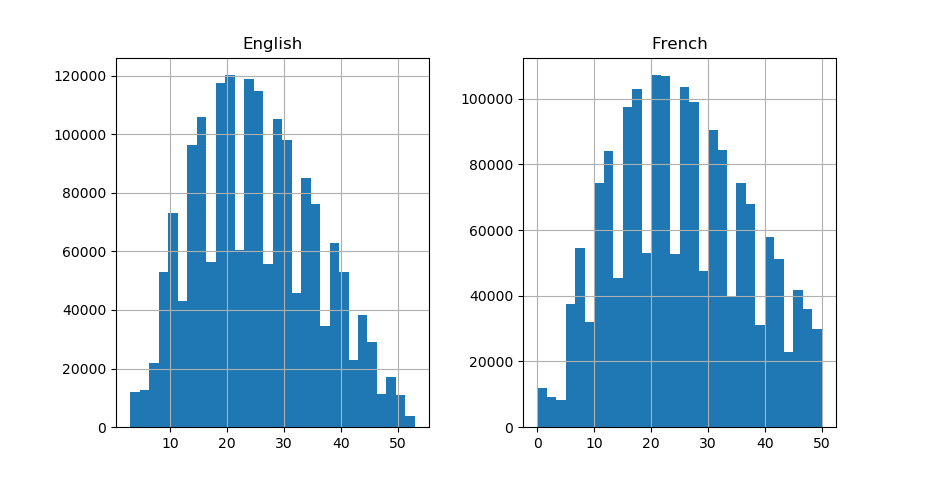
\includegraphics[width=1\textwidth]{media/methodology/sentence-length-chart.png}
\captionsetup{justification=centering,font=Large}
\caption[Diagram of the Europarl dataset sentence length distribution]{Sentence length distribution - Europarl English \& French dataset (\cite{french_corpus_2005}) \\ \textbf{**** ADD X AND Y LABELS TO THE CHART ****}}
\label{fig:sentence_length}
\end{figure}

In contrast, there is very little high quality parallel Scottish Gaelic data readily available. A large percentage of the original Scottish Gaelic data is technical information which contains a lot of software specific keywords, links and technical jargon. This is not ideal reference material for \acrshort{NMT} training data as it leads to a huge vocabulary size where the majority of words appear very few times and do not form coherent sentences, rather short descriptors of the field they represent in the respective localisation file. 

The LearnGaelic data was extracted from learning materials on the \cite{learn_gaelic_2019} website. PDFs are provided on a static template with the English text on one side and the Gaelic version of the same text on the other. Converting these PDFs into the HTML format allowed the data to be categorised and extracted into individual text files while retaining the original alignment of sentences between English and Gaelic.
Despite the low quantity of data from the LearnGaelic source, this data could be considered the highest quality as it is consists of a diverse set of conversations that are quite informal and natural. Similarly, the original Tatoeba datasets consist of concise, natural sentences that have been manually translated and aligned by an online community of translators.

The composition of the data corpus can have a significant impact on the results of the translation quality evaluation. Should the entire training corpus be of a similar context, structure, and limited vocabulary, evaluations on the test set can be inflated due to their similarity with the training set.
To create a varied data corpus in the low-resource context, a subset of samples that do not exceed the maximum sentence length from the multiple datasets totalling 160,000 have been selected to construct the core dataset for the \acrshort{NMT} models. The sources selected for this dataset can be seen in table \ref{tab:low_resource-data}.

\begin{table}[!ht]
\centering
\begin{tabular}{|l|l|}
\hline
\multicolumn{1}{|c|}{\textbf{Quantity}} & \multicolumn{1}{|c|}{\textbf{Source}} \\ \hline
62,000  & Tatoeba German (\cite{tatoeba_data_2020}) \\ \hline % 113,500
62,000  & Udacity French (\cite{udacity_data_2020}) \\ \hline % 104,000
32,500  & Tatoeba Finnish (\cite{udacity_data_2020}) \\ \hline % 32,950
1,800   & Tatoeba Irish (\cite{tatoeba_data_2020}) \\ \hline
800     & LearnGaelic (\cite{learn_gaelic_2019}) \\ \hline
900     & Tatoeba Gaelic (\cite{tatoeba_data_2020}) \\ \hline
\end{tabular}
\captionsetup{justification=centering,font=Large}
\caption{Back-translated data augmentation}
\label{tab:low_resource-data}
\end{table}

\subsection{Pre-processing}

A series of data cleaning and processing is required to ensure the consistency of the data structure throughout the dataset. Subsequently, tokenization will convert the data into sequences of word indices that can be understood by the \acrshort{NMT} models. This includes the following steps:

Data Cleaning:
\begin{itemize}
    \item Convert all characters to lowercase and from Unicode to ASCII. % Why ASCII???
    \item Replace all characters outwith [a-z, ".", "?", "!", ","]
    \item Insert a space between words and punctuation
    \item Truncate consecutive character spacing
    \item Exclude sentence pairs that exceed the maximum word limit
\end{itemize}

Data Processing:
\begin{itemize}
    \item Add <start> and <end> string delimiters to target sentences
    \item Enforce the vocabulary limit, prioritising most frequent words
    \item Word replacement for out of vocabulary or below minimum occurrence threshold
    \item Tokenize the source and target sentences using their vocabularies
\end{itemize}

\section{Frameworks}
\label{sec:3-frameworks}
% Keras
% create models, one hot encoding, tokenizer, padding
% add reference for Tensorflow and Keras

Tensorflow (\cite{tensorflow_2015}) is an open source library for machine learning that provides the framework for the development of neural networks in Python.
Keras (\cite{keras_2015}) is a high-level API for Tensorflow that encapsulates the complexities through a simplified interface.
For this project, Keras has been used for a variety of essential machine learning steps such as padding variable length sequences, one-hot encoding, model implementation and the training and inference methods described in Section \ref{sec:3-model}.

% Numpy / pandas
% manipulate data (reshape etc).

%\section{Architectures Considered}
%\ref{sec:3-architectures}

%\subsection{Long Short-Term Memory}

%\subsection{Gated Recurrent Unit}



\section{Model}
\label{sec:3-model}
\subsection{Parameters}

% reference about importance of parameter tuning
Parameter tuning can have a big impact on the quality of translation model efficiency, speed, and quality so it is essential that a wide variety of parameters are available. The parameters for this project are stored in a separate parameters file that is linked to the runtime of experiments to store the relevant state of the parameters per experiment. The key parameters that are available for tuning are shown in table \ref{tab:model-parameters} along with a description of their purpose.

%\begin{table}[!ht]
%\centering


\begin{table}[!ht]
\centering
\small
\begin{tabular}{|l|p{6.6cm}|l|}
\hline
\multicolumn{1}{|c|}{\textbf{Parameter}} & \multicolumn{1}{c|}{\textbf{Description}}                                       & \textbf{Example} \\ \hline
BATCH\_SIZE                & Batch size of the \acrshort{GRU} inputs            & 64    \\ \hline
HIDDEN\_UNITS              & Number of hidden units in the \acrshort{GRU}       & 128   \\ \hline
LEARNING\_RATE             & Learning rate of the optimiser                     & 0.001 \\ \hline
DROPOUT\_W                 & Dropout rate                                       & 0.2   \\ \hline
DROPOUT\_U                 & Recurrent dropout rate                             & 0.2   \\ \hline
SOURCE\_TIMESTEPS          & Number of timesteps for the source language        & 20    \\ \hline
TARGET\_TIMESTEPS          & Number of timesteps for the target language        & 20    \\ \hline
TEST\_SPLIT                & Training / test data split                         & 0.2   \\ \hline
VALIDATION\_SPLIT          & Training / validation data split                   & 0.2   \\ \hline
MAX\_WORDS\_PER\_SENTENCE  & Maximum number of words in a sentence              & 20    \\ \hline
MIN\_WORD\_OCCURRENCE      & Minimum number of occurrences to be included in vocabulary & 5 \\ \hline
FORCE\_SOURCE\_VOCAB\_SIZE & Source language vocabulary size limit              & 2500 \\ \hline
FORCE\_TARGET\_VOCAB\_SIZE & Target language vocabulary size limit              & 2500 \\ \hline
\end{tabular}
\captionsetup{justification=centering,font=Large}
\caption{Model Parameters}
\label{tab:model-parameters}
\end{table}

\subsection{Architecture}

% back up this with an image of the architecture
The full model consists of a source input layer, encoder \acrshort{GRU}, attention layer, target input layer, decoder \acrshort{GRU}, concatenate layer, and time distributed dense layer.

The model uses a Bahdanau attention layer (\cite{bahdanau_neural_2016}), where the encoder and decoder hidden states are searched for the most relevant information.
The concatenate layer receives input in the form of tensors from the decoder \acrshort{GRU} and attention layer, concatenating them and outputting a single tensor. Finally, the time distributed dense layer applies the fully connected dense layer to every timestep in the \acrshort{GRU}.



\begin{figure}[ht!]
\centering
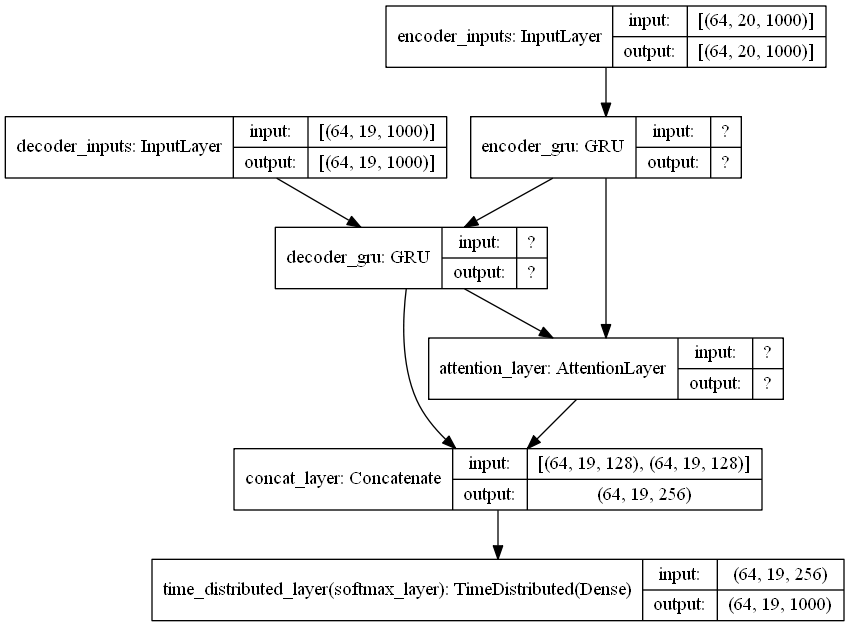
\includegraphics[width=1\textwidth]{media/methodology/model_diagram.png}
\captionsetup{justification=centering,font=Large}
\caption[Diagram of the model architecture]{Model Architecture \\ \textbf{**** Temporary model diagram - replace with a nice diagram ****}}
\label{fig:model_diagram}
\end{figure}



\subsection{Training}
% Talk about training on GPU rather than GPU and the performance benefits in terms of speed
Training neural networks on Tensorflow is possible on both a GPU and a CPU. Due to fundamental hardware differences between the two such as memory bandwidth and memory access latency, using a GPU can accelerate the training of models with a large datasets. To take advantage of the increased computational efficiency and reduction in training time, all of the training conducted during experimentation was done using Tensorflow GPU.
% can add a reference for GPU speed training

Given the hardware constraints of a GTX 1070 8GB graphics card, the model has a batch size of 64 and has 128 hidden units. This ensures that the video memory resources will not be exhausted and interrupt training. Had more resources been available, the parameters identified in the transfer learning literature would be replicated (256 batch size and 1000 hidden units). This would significantly increase the number of trainable parameters which means that the network has more flexibility in representing the desired mapping.

The models are trained using the Adam optimizer (\cite{adam_optimizer_2014}) with a learning rate of 0.001 and the categorical cross-entropy loss function. To help prevent overfitting during early epochs and improve generalisation of the models, dropout and recurrent dropout has been applied to the encoder \acrshort{GRU} and decoder \acrshort{GRU} with a value of $0.2$.

The full model, encoder model, and decoder model are all saved at the end of an epoch if the mean validation loss of the epoch improves upon the previous best validation loss. If no improvements are observed after 5 epochs then training is stopped.


Along with the full model, an inference encoder and decoder model are defined during initialisation. The inference models are used to predict the translation of source sentences into the target language. Separate models are required because the full model expects an input from the source and target language. In contrast, during inference a single input from the source language is received and an output in the target language is inferred. As well as the output translation, attention weights are also saved during inference.

\section{Transfer Learning}
\label{sec:3-transfer_learning}

The experiments investigate the use of both trivial transfer learning and hierarchical transfer learning to take advantage of the knowledge gained on a high-resource language, initialising the low-resource language in an effort to improve translation quality as identified in the literature review (Section \ref{sec:2-transfer_learning}).

% Talk about size of parent dataset
The high-resource languages that have been selected for use in transfer learning are French, Italian, and Irish Gaelic. In theory, Irish Gaelic as an intermediary language for hierarchical transfer learning should help transform the French word embeddings closer to a representation that better fits the syntactic structure of the low-resource language Scottish Gaelic. However in practise, it is unclear whether the relatedness of Irish Gaelic and Scottish Gaelic may exceed the performance of a Tatoeba dataset as an intermediary or parent language for transfer-learning due to the higher quality of the dataset.

% Talk about vocabulary size, minimum word replacement
When a model is defined, the vocabulary size of the source language and the target language is used as a parameter to define the shape of encoder and decoder \acrshort{GRU}. High-resource languages will typically have a much higher vocabulary size by default given there are many more training examples. A vocabulary size limit is required for transfer learning as the input shape that is passed to the encoder and decoder must be the same as the initial declaration. The limitation means that these vocabulary sizes remain consistent between different languages and datasets.

The vocabulary size has been restricted to 10,000 for all languages used in the experiments, replacing words outside of this limit with the out of vocabulary unknown word token "UNK". The implementation of this restriction prioritises the most frequently occurring words by sorting them by frequency in descending order and adding up to 10,000 words to the vocabulary dictionary.
In addition to the vocabulary size limit, a minimum word replacement can be specified with the purpose of removing words that only occur in a very small subset of training samples. Given the limited vocabulary size present in the low-resource language training dataset, this value remains at 2 for the duration of the experiments that use the Scottish Gaelic data. Had this been increased, the vocabulary size would not reach the aforementioned vocabulary size enforcement value of 10,000. For the high-resource languages, despite a minimum word replacement value of 2, as a result of the limited vocabulary size, most if not all of the training samples will significantly exceed this value.

% Make a graphic representing the vocabulary count occurrences for each language (french, irish, gaelic). Will be interesting to see what the distribution of the counts are given the minimum word occurrence set to 2.


\section{Evaluating Translations}
\label{sec:3-evaluating}

As identified in the literature review, \acrshort{BLEU} score will be used as the primary metric for the translation evaluation. To ensure the robustness of the results, evaluations will be presented in the form of \acrshort{BLEU}-1 to \acrshort{BLEU}-4. Although a translations may receive a high score for \acrshort{BLEU}-1, there is a significant difference in difficulty for receiving a high \acrshort{BLEU}-4 score as a higher percentage of n-gram counts are required to match the reference translation. The evaluations are calculated using cumulative score rather than individual score as it better represents the metric distribution. 

Another form of evaluation will be in the form of a sentence analysis table. The direct comparison between implementation translations makes it easier to visualise the discrepancies outlined by \acrshort{BLEU} scores.
Finally, an attention plot diagram using the attention weights will help visualise the inner workings of the attention mechanism's influence on the decision making process of the network for output predictions. 
